\documentclass[11pt]{article}

\usepackage[top=1in, bottom=1in, left=1in, right=1in]{geometry}
\usepackage[spanish,activeacute]{babel}
\usepackage{graphicx}

\begin{document}

\title{Trabajo Pr'actico de Inform'atica 2 - Zoz}
\author{Guido Nu'nez}
\maketitle

\begin{enumerate}
	
\item Formulaci'on y an'alisis del problema:	
	
	\begin{enumerate}
	
	\item Escriba la formulaci'on del problema: estados, estado inicial, funci'on sucesora, verificaci'on de la meta y costo del camino. \\
	
	Estados: Un estado es una configuraci'on del tablero con x fichas colocadas, $1<=x<=f(N)-1$, $f(N)$= cantidad de celdas del tablero en funcion a un lado $N$, tal que se haya obtenido mediante un movimiento v'alido o sea la configuraci'on del estado inicial.
	
	Estado inicial: Cualquier configuraci'on del tablero con $f(N)-1$ fichas colocadas.
	
	Funci'on sucesora: Mover una ficha en cualquier direcci'on hacia una celda desocupada pasando exactamente por encima de una ficha intermedia y quitando esta 'ultima del tablero.
	
	Verificaci'on de la meta: Cualquier configuraci'on del tablero con una sola ficha colocada.
	
	Costo del camino: N'umero de pasos. \\
	
	\item Encuentre una formula $f(N)$ que expresa el n'umero de posiciones que tiene el tablero en funci'on a uno de los lados N. Por ejemplo, los tableros ilustrados en las figuras tienen un lado de 5 posiciones, luego existen $f(5) = 15$ posiciones en el tablero. Muestre paso a paso como deduce la 	formula a su expresi'on algebraica m'as sencilla. \\
	
	Un tablero con n celdas por lado puede verse como un tri'angulo con $1+2+3+...+(n-1)+n$ celdas.
	$$f(n)=1+2+...+(n-1)+n$$
	$$f(n)+f(n)=1+2+...+(n-1)+n+n+(n-1)+...+2+1$$
	$$f(n)+f(n)=(1+n)+(2+n-1)+...+(n-1+2)+(n+1)$$
	$$f(n)+f(n)=(n+1)+(n+1)+...+(n+1)+(n+1)$$
	$$2f(n)=n(n+1)$$
	$$f(n)=\frac{n(n+1)}{2}$$ \\
	
	\item En base a la formula $f(N)$ encontrada (Ejercicio 1b), halle el tama'no de los tableros para los lados N = 	\{5; 6; 7; 8; 9; 10\}
	
	\begin{center}
	\begin{tabular}{|c|c|c|c|c|c|c|}
	\hline	
	& $f(5)$ & $f(6)$ & $f(7)$ & $f(8)$ & $f(9)$ & $f(10)$ \\ 			\hline
	Dimensi'on del tablero & 15 & 21 & 28 & 36 & 45 & 55\\ 				\hline
	\end{tabular}
	\end{center} 
	
	\item ?`Cu'al es el tama'no del espacio de estados para el juego Zoz? Una vez derivada la expresi'on, calcule el espacio de estados para dimensiones de tableros cada vez mayores. El tablero inicial puede ser cualquier configuraci'on de fichas en donde exactamente una posici'on del tablero se encuentra libre. Puede asumir que todas las configuraciones del tablero son v'alidas. \\
	
	Dado que para cada $N$ existe una cantidad $f(N)$ de celdas y cada celda puede llevar dos valores (contener o no una ficha), y exceptuando la configuraci'on que contiene todas las celdas vac'ias y la configuraci'on que contiene todas las celdas con fichas, el tama'no del espacio de estados es $2^{f(N)}-2$. 	
	\begin{center}		
	\begin{tabular}{|c|c|c|c|c|c|c|}
	\hline	
	& $N=5$ & $N=6$ & $N=7$ & $N=8$ & $N=9$ & $N=10$ \\ \hline
	Espacio de estados & $32766$ & $2097150$ & $268435454$ & $6.872\times10^{10}$ & $3.518\times10^{13}$ & 					$3.603\times10^{16}$ \\ \hline
	\end{tabular}		
	\end{center} 	
	
	\item Suponga que somos capaces de almacenar cada posici'on del tablero Zoz en un 'unico 'atomo, y que el universo 	visible tiene un total de $10^{80}$ 'atomos en su totalidad. ?`Cu'al es el tablero de lado $N$ m'as grande que se podr'ia resolver en este universo visible? \\
	
	El tablero m'as grande que se podr'ia resolver en este 	universo visible es un tablero con $N=22$, con $1.447\times10^{76}$ 'atomos utilizados. \\
	
	\item Considere que cada posici'on del tablero ocupa 16 bytes en la memoria. >Cu'anta memoria se necesita para cada caso? \\
	
	\begin{tabular}{|c|c|c|c|c|c|c|}
	\hline	
	& $N=5$ & $N=6$ & $N=7$ & $N=8$ & $N=9$ & $N=10$ \\ \hline
	Total de memoria & $524256$ & $33554400$ & $4294967264$ & 			$1.100\times10^{12}$ & $5.629\times10^{14}$ & 						$5.765\times10^{17}$ \\ 
	(en bytes) & & & & & & \\ \hline
	\end{tabular}	

	\end{enumerate}

\item Una vez definido el problema, escriba el programa para resolver el juego Zoz. Halle la soluci'on al problema empleando las siguientes estrategias de b'usqueda:
	\begin{enumerate}
	\item Breadth First Tree Search (BFTS)
	\item Breadth First Graph Search (BFGS)
	\item Uniform Cost Graph Search (UCGS)
	\item Depth First Tree Search (DFTS)
	\item Depth First Graph Search (DFGS)
	\item Recursive Depth First Search (RDFS)
	\item Iterative Deepening Search (IDS)
	\item Greedy Best First Graph Search (GBFGS)
	\item Recursive Greedy Best First Search (RGBFS)
	\item A* (A*S) \\
	\end{enumerate}		

Las soluciones pueden verse ejecutando el programa implementado y siguiendo las instrucciones. \\

\item Eval'ue la complejidad temporal y espacial de cada estrategia de b'usqueda para el problema Zoz de dimensi'on $N = 5$. La complejidad temporal y espacial deben medirse seg'un los criterios presentados en el libro de Russell y Norvig. Con los resultados obtenidos construya una tabla de resultados. \\

\begin{tabular}{|c|c|c|c|}
\hline	
Estrategias de b'usqueda & Complejidad Temporal & Complejidad Espacial & Costo de buscar \\ \hline
(BFTS) & $323872$ & $323873$ & $647745$ \\ \hline
(BFGS) & $4845$ & $4846$ & $9691$ \\ \hline
(UCGS) & $4846$ & $4847$ & $9693$ \\ \hline
(DFTS) & $6281$ & $92$ & $6373$ \\ \hline
(DFGS) & $1102$ & $92$ & $1194$ \\ \hline
(RDFS) & $6281$ & $92$ & $6373$ \\ \hline
(IDS) & $1011045$ & $92$ & $1011137$ \\ \hline
(GBFGS) & $942$ & $943$ & $1885$ \\ \hline
(RGBFS) & $1008$ & $1009$ & $2017$ \\ \hline
(A*S) & $4507$ & $4508$ & $9015$ \\ \hline
\end{tabular}	

\item Una vez elaborada la tabla conteste a las siguentes preguntas:
	\begin{enumerate}
	
	\item ?`C'omo se explican las diferencias en la complejidad temporal y espacial de las estrategias de b'usqueda Breath First Search en la versi'on implementada como 'arbol y grafo? ?`Sucede lo mismo en el caso de Depth First Search?\\
	
	La estrategia de b'usqueda Breadth First Three Search implementada como 'arbol posee una mayor complejidad espacial y temporal que la versi'on implementada como grafo.
	Esto ocurre debido a que la versi'on implementada como grafo mantiene una lista (explored) que almacena los nodos que ya se han expandido y esto evita expandir nodos repetidos. Esto reduce tanto la complejidad temporal como la espacial. Lo mismo ocurre con la estrategia de b'usqueda Depth First Search. \\
	
	\item Describa la heur'istica h() que dise'n'o para implementar la b'usqueda Greedy. \\
	
	La funci'on heur'istica dise'nada busca evitar llegar a estados de los cuales no se puede llegar a un estado meta. En particular consider'e la configuraci'on de tablero en la que las fichas se encuentran colocadas en los bordes y no en las celdas interiores. Esta es una configuraci'on a partir de la cual no se puede avanzar. Bas'andome en esto, la funci'on heur'istica va sumando una unidad por cada ficha colocada en un borde y por cada celda vacia en el interior del tablero. Con esto se logra obtener una suma alta para configuraciones no deseadas y as'i el algoritmo de b'usqueda evita elegir estos estados. \\
	
	\item Describa la heur'istica h() que dise'n'o para implementar la b'usqueda A*. Dada la heur'istica h() dise'nada, ?`la b'usqueda A* es 'optima? \\
	
	La heur'istica utilizada es la misma que la dise'nada para la b'usqueda Greedy. Todas las soluciones de Zoz poseen el mismo costo de camino = 13, por lo que cualquier soluci'on es 'optima, y por lo tanto, la b'usqueda A* es 'optima. \\ 	
	
	\item ?`Las estrategias desinformadas o informadas son mejores para resolver Zoz con $N=5$? \\
	 	
	Las estrategias informadas en conjunto son mejores para resolver Zoz con $N=5$. Sin embargo, estas estrategias no contienen a la mejor estrategia para resolver el juego. Seg'un las experimentaciones realizadas la mejor estrategia es Depth First Graph Search que se encuentra entre las estrategias no informadas. A pesar de esto, las estrategias no informadas no pueden considerarse como mejores debido a las altas complejidades de las dem'as estrategias constituyentes. \\
	
	\item >Las estrategias de b'usqueda en profundidad o en anchura son mejores para resolver Zoz con $N=5$? ?`A qu'e se debe esto? \\
	
	Para resolver Zoz con $N=5$ son mejores las estrategias de b'usqueda en profundidad. Esto se debe a que los nodos metas se encuentran en el nivel 13 del 'arbol y la b'usqueda en anchura debe expandir todos los nodos de cada nivel para llegar a ese nivel. En cambio, la b'usqueda en profundidad no necesita expandir todos los nodos de los niveles inferiores ya que el nodo meta hallado no se encuentra entre las 'ultimas hojas del 'arbol ubicadas m'as a la derecha. \\ 
	
	\item ?`Cu'al es el mejor algoritmo de b'usqueda para Zoz con $N=5$? ?`Se puede afirmar tambi'en que es el mejor para dimensiones mayores $N>5$? \\
	
	La mejor estrategia es Depth First Graph Search debido a que obtiene el menor costo de buscar gracias a una baja complejidad temporal y espacial. Se puede considerar que es la mejor tambi'en para dimensiones mayores ya que por m'as que que no obtenga la mejor complejidad temporal (alguna estrategia informada podr'ia tener una mejor), es la que necesitar'ia menos memoria. \\
	
	\item Usted es un investigador que quiere contribuir con la ciencia encontrando mejores algoritmos de b'usqueda para resolver el juego Zoz. Dados los resultados experimentales que obtuvo, ?`Qu'e tipo de algoritmos de b'usqueda se 	esforzar'ia en investigar a continuaci'on? \\
	
	Investigar'ia estrategias informadas, ya sea Greedy o A*, debido a las dependencias de 'estas sobre las funciones heur'isticas. Tratar'ia de hallar heur'isticas admisibles y consistentes que permitan reducir las complejidades de estas estrategias, como tambi'en ciertas mejoras o cambios que puedan aplicarse a dichas estrategias de modo a obtener el m'aximo provecho de ellas. \\
	
	\end{enumerate}

\item ?`Es posible utilizar la b'usqueda bidireccional para este problema? En caso afirmativo, escriba la funci'on
predecesora. \\

Si, es posible, construyendo un nuevo estado ficticio cuyos predecedores inmediatos son los estados meta del juego.
El estado ficticio que utilic'e corresponde a una configuraci'on de tablero con todas las celdas vac'ias. Los predecesores de este estado ficticio son los estados cuyas configuraciones de tablero poseen una 'unica ficha colocada.
La funci'on predecesora puede verse en el c'odigo del trabajo, dentro de la definici'on del problema Zoz y puede ejecutarse ejecutando el programa implementado y siguiendo las instrucciones.
	
	 
\item ?`Cualquier configuraci'on inicial de fichas sobre el tablero sirve para jugar este juego? Implemente una
funci'on que lo prueba. \\

Para un tablero con $N=5$, cualquier configuraci'on inicial de fichas sirve para jugar el juego. La prueba puede observarse ejecutando el programa implementado y siguiendo las instrucciones. \\

\item ?`Cu'al es la instancia de problema m'as grande (N) que pudiste resolver? >Cu'al es el algoritmo de
b'usqueda que elegiste para intentar resolver instancias m'as grandes del problema? ?`Con qu'e criterio
elegiste el algoritmo de b'usqueda? \\ 

La instancia m'as grande que pude resolver fu'e con $N=6$ para una HP Pavilion dv4 Notebook PC, con procesador AMD Turion(tm) II Dual-Core Mobile M500 2.20 GHz y memoria de 4 GB. Prob'e una instancia con $N=7$ durante 6 horas sin lograr resultado alguno. El algoritmo utilizado fu'e el Depth First Graph Search debido a que es el mejor algoritmo de b'usqueda para Zoz seg'un lo establecido anteriormente. \\

\item ?`Cu'ales son las caracter'isticas del 'arbol de b'usqueda completo? Utilice el algorimo Breadth First Tree
Search (BFTS) con $N=5$ para completar la tabla a continuaci'on:

\begin{center}
\begin{tabular}{|c|c|}
\hline	
Dimensi'on completa del arbol & $N=5$ \\ \hline
M'aximo factor de anchura (b) & 8\\ \hline
M'axima profundidad del 'arbol (m) & 13\\ \hline
Total de nodos que tiene el 'arbol & 823873\\ \hline
Total de soluciones que tiene Zoz & 1550\\ \hline
\end{tabular}	
\end{center}

?`Coincide el espacio de estados para $N=5$ (calculado en el Ejercicio 1d) con el total de nodos que tiene 'arbol? Explique. \\

No coincide. Esto ocurre debido a que los nodos del 'arbol poseen estados repetidos. El espacio de estados no tiene en cuenta los estados repetidos. Por ende el total de nodos del 'arbol es mayor al espacio de estados. \\

\item El programa que implementaste es un:
	\begin{itemize}
	\item Agente reflejo
	\item Agente basado en memoria
	\item Agente basado en metas
	\item Agente basado en utilidades
	\item Agente que aprende
	\item Ninguna de las anteriores
	\end{itemize}
	Elija la opci'on m'as acertada para el trabajo que 					entregaste. \\
	
Es una clase de agente basado en metas llamado agente resolvente-problemas. Los agentes resolventes-problemas deciden qu'e hacer para encontrar secuencias de acciones que conduzcan a estados deseables.

\end{enumerate}

\newpage

\begin{flushleft}
Observaciones para la ejecuci'on del programa: 
\end{flushleft}

\begin{flushleft}
Para la ejecuci'on del programa solo es necesario ejecutar el archivo zoz.py y luego seguir las indicaciones.
Si el programa pide introducir el valor de fila y columna de la celda para el estado inicial, se introduce valores seg'un la siguiente la siguiente imagen:
\end{flushleft}

\begin{center}
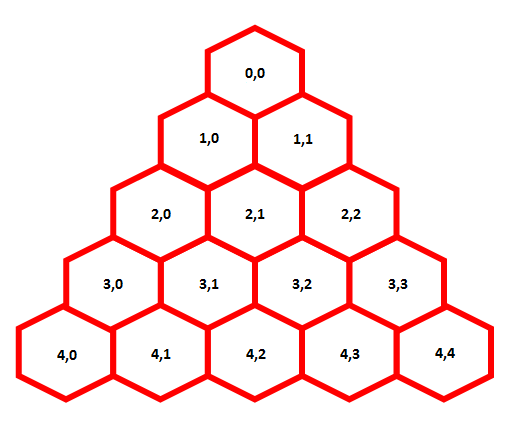
\includegraphics{tablero.png}
\end{center}

\end{document}